% Full instructions available at:
% https://github.com/elauksap/focus-beamertheme

\documentclass{beamer}
\usetheme[numbering=progressbar, nofirafonts]{focus}
\definecolor{main}{RGB}{10,20,43}
\definecolor{background}{RGB}{255,255,255}

\title{Scooter Trajectories Clustering}
\subtitle{Machine Learning and Deep Learning}
\author{Mirco De Marchi VR445319}
%\titlegraphic{\includegraphics[scale=1.25]{focus-logo.pdf}}
\institute{University of Verona}
\date{2020/2021}

\usepackage{amsmath}

\usepackage{graphicx}
\graphicspath{ {../../image/} }

\usepackage{tikz}
\usetikzlibrary{positioning,shapes,shadows,arrows}

\usepackage{multicol}
%\setlength{\multicolsep}{6.0pt plus 2.0pt minus 1.5pt}% 50% of original values
\setlength\multicolsep{0pt}

% Disable section frame.
%\AtBeginSection[]{} 

\begin{document}

\begin{frame}
\maketitle
\end{frame}

%\begin{frame}
%\frametitle{Contents}
%\tableofcontents
%\end{frame}

% Use starred version (e.g. \section*{Section name})
% to disable (sub)section page.}
\section{Introduction}

\begin{frame}{Motivation}
 Trajectories clustering is a problem really difficult to be treated but  can be useful for several applications:
 \begin{itemize}
 	\item Monitoring
 	\item Forecasting
 	\item Viability
 	\item Smart City
 	\item Security
 \end{itemize}
\end{frame}

\begin{frame}{State of art}
The current researches can be divided into 5 categories:
\begin{itemize}
	\item Spatial based clustering: \textit{DBSCAN} algorithm.
	\item Time depended clustering: \textit{OPTICS} algorithm.
	\item Partition and group based clustering: \textit{Lee partition \& group}.
	\item Uncertain trajectory clustering: \textit{Fuzzy C-Means} algorithm.
	\item Semantic trajectory clustering: \textit{Stops and Moves} model.
\end{itemize}
\end{frame}

\begin{frame}{Starting point}
Dataset weighs: \textbf{2GB}.
\begin{figure}[bt]
	\centering
	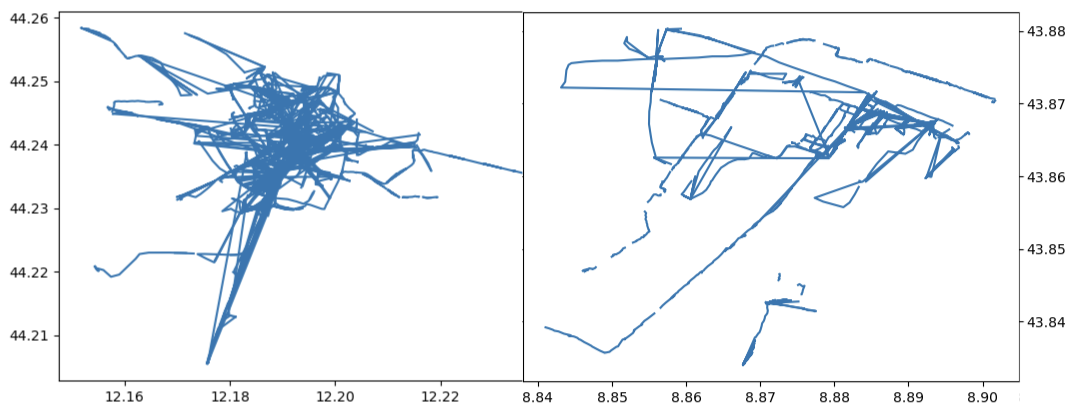
\includegraphics[width=\textwidth]{starting-point}
	\label{fig:starting-point}
	\caption{Rentals showed: 200.}
\end{figure}
\end{frame}

\begin{frame}{Original dataset diagram}
Dataset entities: position, rental, device and user. The dataset has been previously processed in order to delete sensitive informations.
\begin{figure}
	\centering
	\label{original-dataset-diagram}
	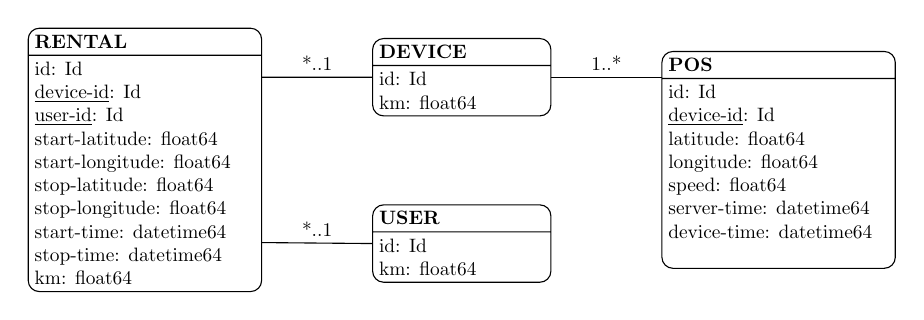
\begin{tikzpicture}[node distance=2cm, scale=0.7, transform shape]
	\node (rental) [rectangle, draw=black, rounded corners, text justified, text width=4cm, rectangle split, rectangle split parts=2]
	{
		\textbf{RENTAL}
		\nodepart{second}
		id: Id\\
		\underline{device-id}: Id\\
		\underline{user-id}: Id\\
		start-latitude: float64\\
		start-longitude: float64\\
		stop-latitude: float64\\
		stop-longitude: float64\\
		start-time: datetime64\\
		stop-time: datetime64\\
		km: float64
	};
	\node (device) [rectangle, draw=black, rounded corners, text justified, text width=3cm, rectangle split, rectangle split parts=2, right=of rental, yshift=1.5cm]
	{
		\textbf{DEVICE}
		\nodepart{second}
		id: Id\\
		km: float64
	};
	\node (pos) [rectangle, draw=black, rounded corners, text justified, text width=4cm, rectangle split, rectangle split parts=2, right=of device, yshift=-1.5cm]
	{
		\textbf{POS}
		\nodepart{second}
		id: Id\\
		\underline{device-id}: Id\\
		latitude: float64\\
		longitude: float64\\
		speed: float64\\
		server-time: datetime64\\
		device-time: datetime64\\
	};
	\node (user) [rectangle, draw=black, rounded corners, text justified, text width=3cm, rectangle split, rectangle split parts=2, below=of device, yshift=0.4cm]
	{
		\textbf{USER}
		\nodepart{second}
		id: Id\\
		km: float64
	};
	
	\draw ([yshift=1.5cm]rental.east) -- node[above]{*..1}  (device.west);
	\draw ([yshift=-1.5cm]rental.east) -- node[above]{*..1} (user.west);
	\draw (device.east) -- node[above]{1..*} ([yshift=1.5cm]pos.west);
	\end{tikzpicture}
\end{figure}
\end{frame}

\section{Methodology}
\begin{frame}{Generated dataset diagram}
\begin{table}
	\centering
	\begin{tabular}{ l r r }
		\hline
		Dataset & Samples & Features \\ \hline
		rental & 14826 & 10 \\ 
		pos & 817076 & 18 \\ 
		merge & 817076 & 18 \\
		dataset & 14826 & 13 \\
		partition city 1 & 608251 & 18 \\
		partition city 2 & 202795 & 18 \\ \hline
	\end{tabular}
\end{table}
\begin{figure}
	\centering
	\label{generated-dataset-diagram}
	\begin{tikzpicture}[node distance=2cm, scale=0.5, transform shape]
	\node (rental) [rectangle, draw=black, rounded corners, text justified, text width=4cm, rectangle split, rectangle split parts=2]
	{
		\textbf{RENTAL}
		\nodepart{second}
		id: Id\\
		\underline{device-id}: Id\\
		\underline{user-id}: Id\\
		start-latitude: float64\\
		start-longitude: float64\\
		stop-latitude: float64\\
		stop-longitude: float64\\
		start-time: datetime64\\
		stop-time: datetime64\\
		km: float64
	};
	\node (pos) [rectangle, draw=black, rounded corners, text justified, text width=10cm, rectangle split, rectangle split parts=2, right=of rental]
	{
		\textbf{POS}
		\nodepart{second}\begin{multicols*}{2}
		id: Id\\
		\underline{rental-id}: Id\\
		timedelta-id: Id\\
		spreaddelta-id: Id\\
		edgedelta-id: Id\\
		coorddelta-id: Id\\
		latitude: float64\\
		longitude: float64\\
		spread-latitude: float64\\
		spread-longitude: float64\\
		\vfill
		\columnbreak
		edge-latitude-start: float64\\
		edge-latitude-stop: float64\\
		edge-longitude-start: float64\\
		edge-longitude-stop: float64\\
		speed: float64\\
		server-time: datetime64\\
		device-time: datetime64\\
		time-gap: float64\\
		\end{multicols*}
	};
	\node (device) [rectangle, draw=black, rounded corners, text justified, text width=3cm, rectangle split, rectangle split parts=2, left=of rental, yshift=1.5cm]
	{
		\textbf{DEVICE}
		\nodepart{second}
		id: Id\\
		km: float64
	};
	\node (user) [rectangle, draw=black, rounded corners, text justified, text width=3cm, rectangle split, rectangle split parts=2, left=of rental, yshift=-1.5cm]
	{
		\textbf{USER}
		\nodepart{second}
		id: Id\\
		km: float64
	};
	
	\draw ([yshift=1.5cm]rental.west) -- node[above]{1..1}  (device.east);
	\draw ([yshift=-1.5cm]rental.west) -- node[above]{ 1..*} (user.east);
	\draw (rental.east) -- node[above]{1..*} (pos.west);
	\end{tikzpicture}
\end{figure}
\end{frame}

\begin{frame}{Rentals trajectories}
\begin{figure}[bt]
	\centering
	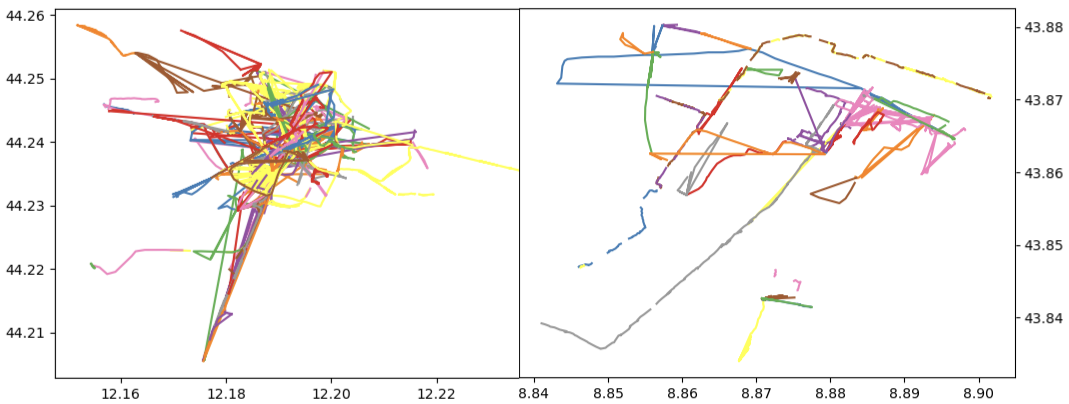
\includegraphics[width=\textwidth]{rental-plot}
	\label{fig:rental-plot}
	\caption{Rentals showed in the 2 cities: 200 (left), 50 (right).}
\end{figure}
\end{frame}

\begin{frame}{Heuristics: \textit{timedelta} and \textit{spreaddelta}}
The following heuristics methodologies use a \texttt{delta} value that is values with the statistic's empirical rule.
\begin{itemize}
	\item \textbf{timedelta heuristic}: a rental trajectory can be divided in a sequence of trajectories if the time gap between a position and previous one exceeds a \textit{timedelta} value.
	\begin{align}
	TIMEGAPS = \{p.time - p[-1].time \mid \forall p \in POS \}
	\end{align}
	\item \textbf{spreaddelta heuristic}: a rental trajectory is similar to another one if they spread a similar amount of area. 
	\begin{align}
	SPREADS = \{max(t) - min(t) \mid \forall t \in TRAJ \}
	\end{align}
\end{itemize}
\end{frame}

\begin{frame}{Heuristics: \textit{edgedelta} and \textit{coorddelta}}
\begin{itemize}
	\item \textbf{edgedelta heuristic}: acts as the \textit{spreaddelta heuristic}, but it considers the edges of a trajectory, or rather the first position and the last position of a trajectory. The main issue is the bimodal distribution of edges.
	\begin{align}
	EDGES = \{concat(p[0], p[-1]) \mid \forall t \in TRAJ \}
	\end{align}
	\item \textbf{coorddelta heuristic}: combination of spread and edge heuristics in order to combine the main advantages. 
\end{itemize}
\end{frame}

\begin{frame}{Position distributions}
The positions are concentrated in 2 distant cities:
\begin{figure}[bt]
	\centering
	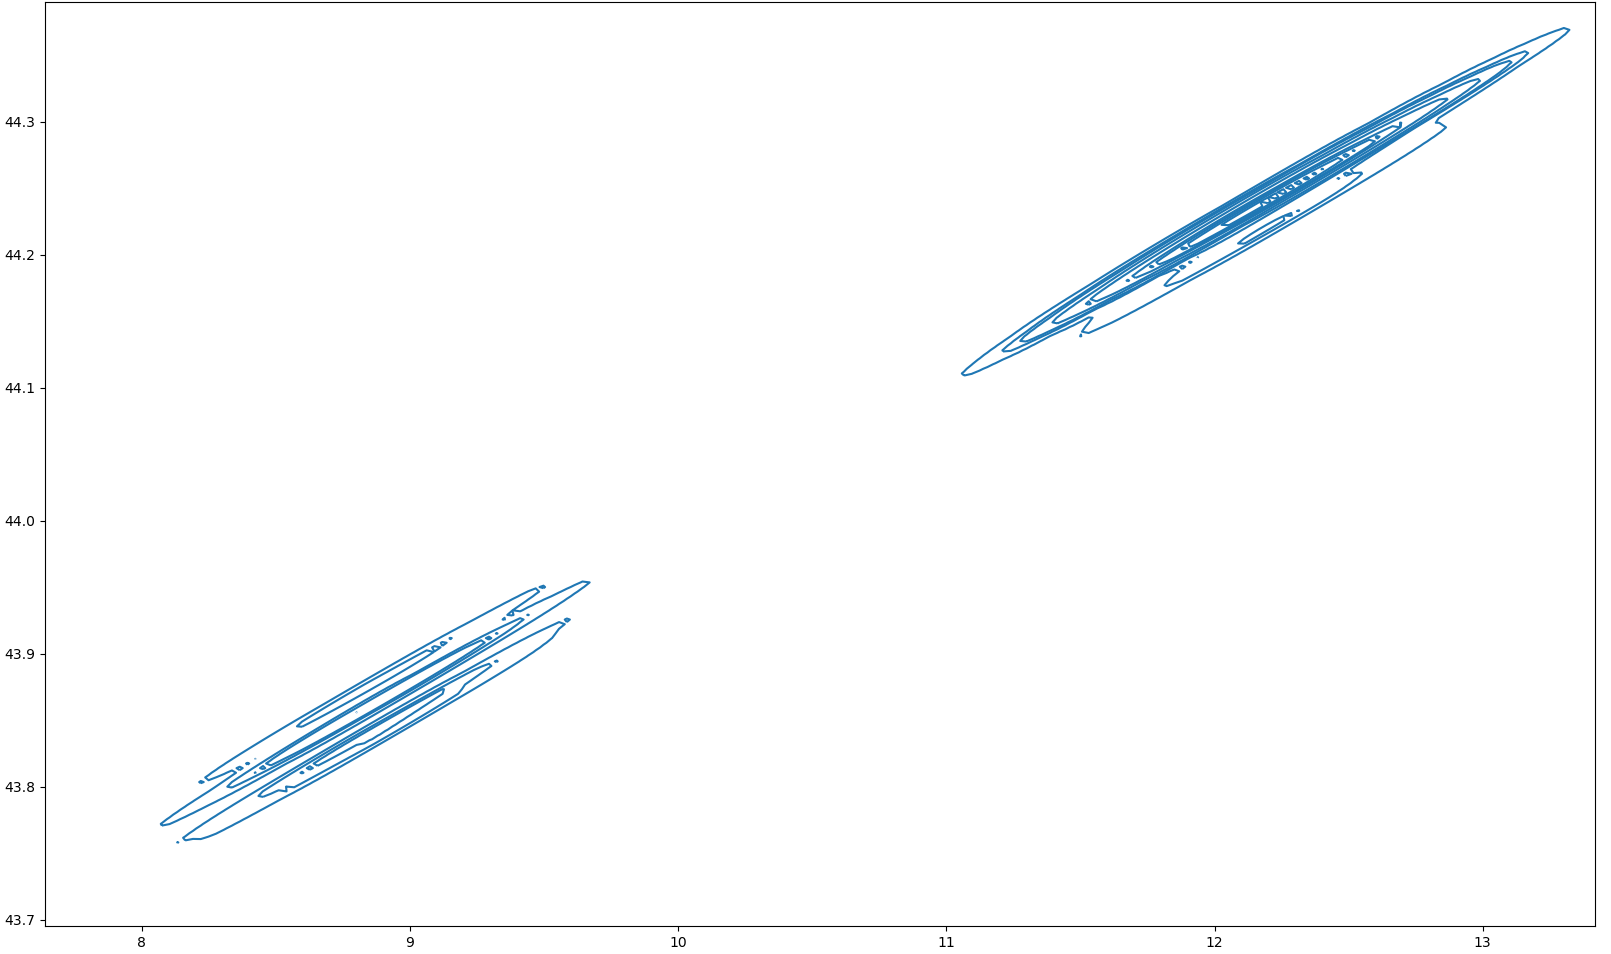
\includegraphics[width=\textwidth]{pos-distributions}
	\label{fig:pos-distributions}
\end{figure}
\end{frame}

\begin{frame}{Feature extraction}
Pipeline: integration of heuristic data as features, \textit{Standardization}, \textit{Normalization} and than \textit{Principal Component Analysis (PCA)}. 
\vfill
The component extracted by \textit{PCA} can be decided in 3 different ways:
\begin{itemize}
	\item By a number a priori;
	\item By the cumulative variance with $80\%$ cover;
	\item Concatenation of columns produced by \textit{PCA} for different subset of features;
\end{itemize}
\end{frame}

\begin{frame}{Clustering}
\begin{itemize}
	\item \textbf{K-Means}: simple technique with distance based metric, fast and cheap in memory terms. $O(n*k*l)$
	\item \textbf{Mean Shift}: density based, automatically sets the number of clusters, but it needs a bandwidth parameter. $O(n ^ 2)$
	\item \textbf{Gaussian Mixture}: estimation of linear combination of a finite number of Gaussian distributions with unknown parameters and \textit{expectation-maximization (EM)} algorithm. $O(l * n ^ 3)$
	\item \textbf{Full Hierarchy Agglomerative}: hierarchical clustering with bottom up approach and minimization metric on the maximum distance between observations in pairs of clusters. $O(n ^ 3)$
	\item \textbf{Ward Hierarchy Agglomerative}: hierarchical clustering with bottom up approach and minimization metric on the sum of squared differences between all clusters. $O(n ^ 3)$
\end{itemize}
\end{frame}

\section{Results}
\begin{frame}{Timedelta heuristic results}
\begin{columns}[t, onlytextwidth]
	\column{0.4\textwidth}
	\begin{figure}[bt]
		\centering
		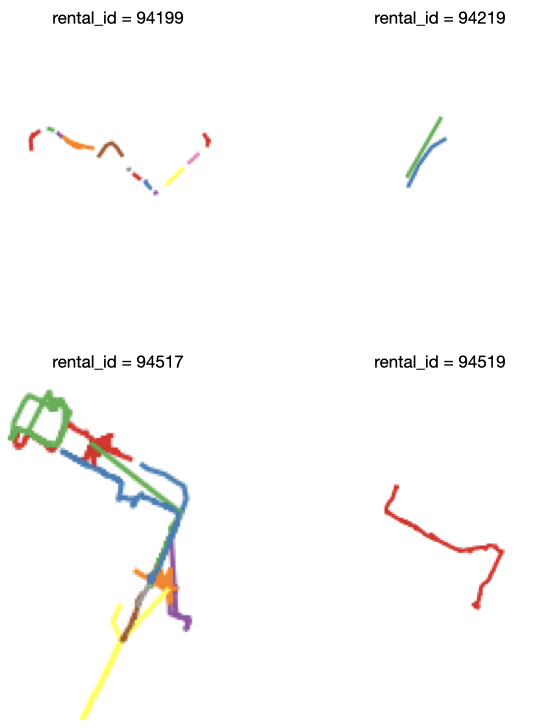
\includegraphics[width=\textwidth]{timedelta-result}
		\label{fig:timedelta-result}
	\end{figure}
	\column{0.6\textwidth}
	\begin{figure}[bt]
		\centering
		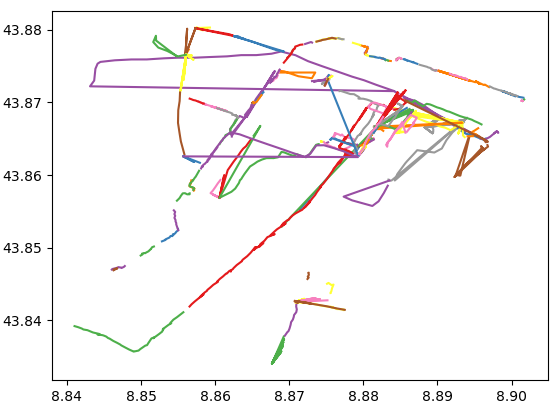
\includegraphics[width=\textwidth]{timedelta-lineplot}
		\label{fig:timedelta-lineplot}
		\caption{Rentals showed: 50.}
	\end{figure}
\end{columns}
\end{frame}

\begin{frame}{Spreaddelta heuristic results}
	\begin{figure}[bt]
		\centering
		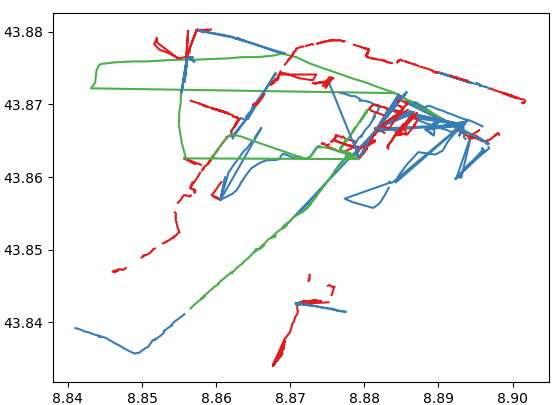
\includegraphics[width=0.85\textwidth]{spreaddelta-result}
		\label{fig:spreaddelta-result}
		\caption{Rentals showed: 50.}
	\end{figure}
\end{frame}

\begin{frame}{Edgedelta heuristic results}
\begin{figure}[bt]
	\centering
	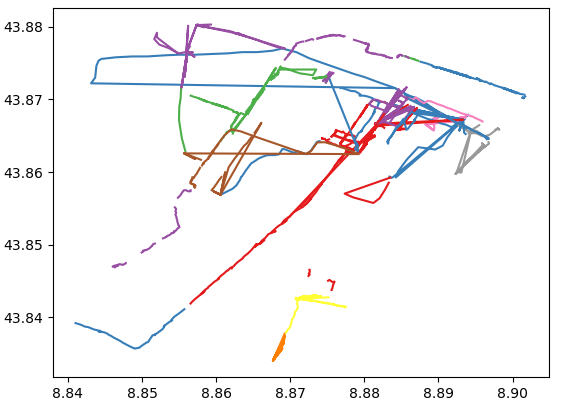
\includegraphics[width=0.85\textwidth]{edgedelta-result}
	\label{fig:edgedelta-result}
	\caption{Rentals showed: 50.}
\end{figure}
\end{frame}

\begin{frame}{Coorddelta heuristic results}
\begin{figure}[bt]
	\centering
	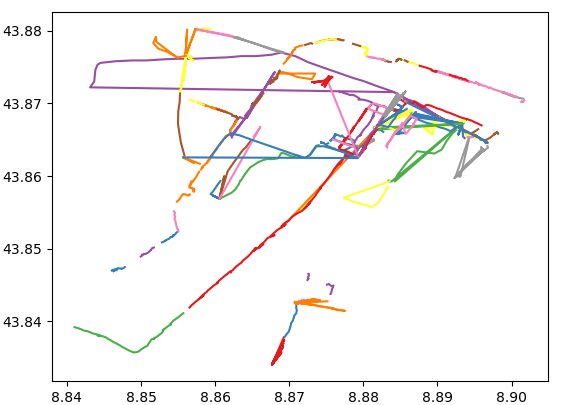
\includegraphics[width=0.85\textwidth]{coorddelta-result}
	\label{fig:coorddelta-result}
	\caption{Rentals showed: 50.}
\end{figure}
\end{frame}

\begin{frame}{WCSS and Elbow method}
\textit{Within Cluster Sum of Squares (WCSS)} graph for \textit{Elbow method} in range from 1 to 30 with K-Means
\begin{figure}[bt]
	\centering
	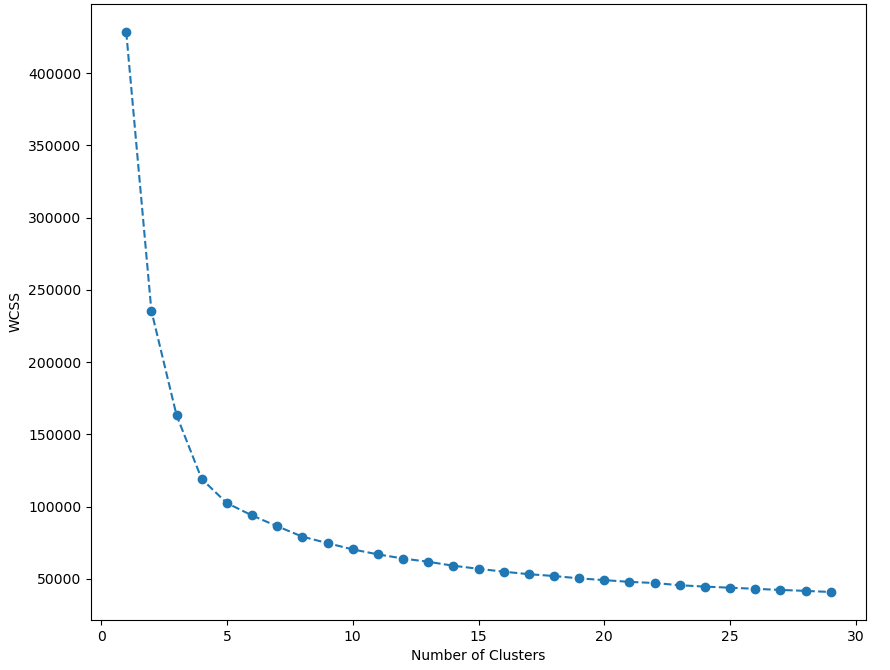
\includegraphics[width=0.6\textwidth]{wcss}
	\label{fig:wcss}
\end{figure}
Number of clusters estimated: \textbf{5}.
\end{frame}

\begin{frame}{Gaussian Mixture clustering}
\begin{figure}[bt]
	\centering
	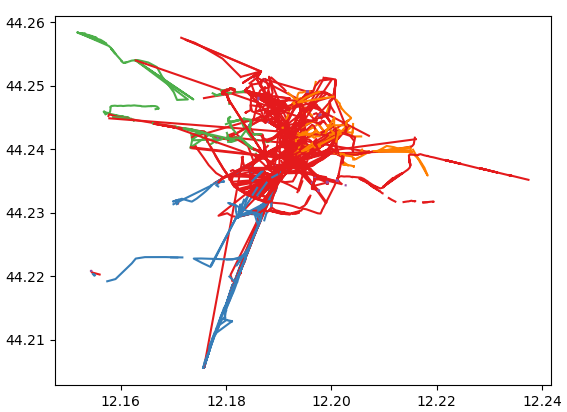
\includegraphics[width=0.85\textwidth]{gaussian-mixture-plot}
	\caption{Silhouette: -0.02. Rentals showed: 200.}
	\label{fig:gaussian-mixture-line}
\end{figure}
\end{frame}

\begin{frame}{Mean Shift clustering}
\begin{figure}[bt]
	\centering
	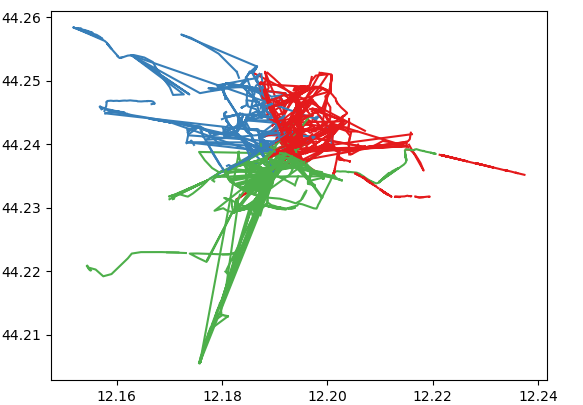
\includegraphics[width=0.85\textwidth]{mean-shift-plot}
	\caption{Silhouette: 0.40. Rentals showed: 200.}
	\label{fig:mean-shift-line}
\end{figure}
\end{frame}

\begin{frame}{Full Hierarchical Agglomerative}
\begin{columns}[t, onlytextwidth]
	\column{0.7\textwidth}
	\begin{figure}[bt]
		\centering
		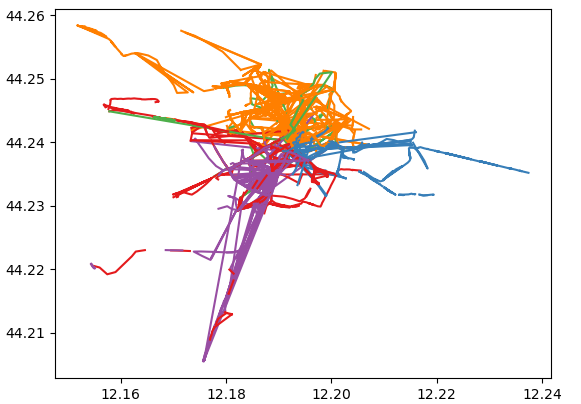
\includegraphics[width=\textwidth]{full-agglomerative-plot}
		\caption{Silhouette: 0.16. Rentals showed: 200.}
		\label{fig:full-agglomerative-line}
	\end{figure}
	\column{0.3\textwidth}
	\begin{figure}[bt]
		\centering
		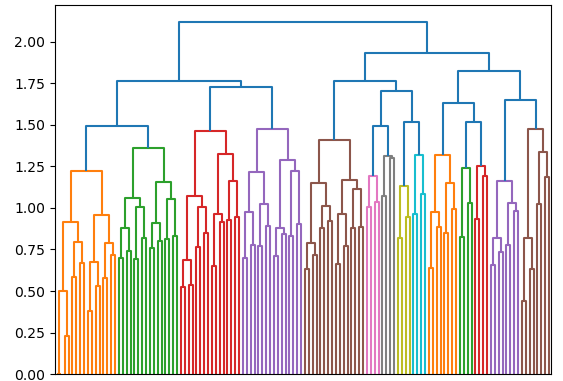
\includegraphics[width=\textwidth]{full-agglomerative-dendrogram}
		\caption{Dendrogram up to level 5 of merge}
		\label{fig:full-agglomerative-dendrogram}
	\end{figure}
\end{columns}
\end{frame}

\begin{frame}{Ward Hierarchical Agglomerative}
\begin{columns}[t, onlytextwidth]
	\column{0.7\textwidth}
	\begin{figure}[bt]
		\centering
		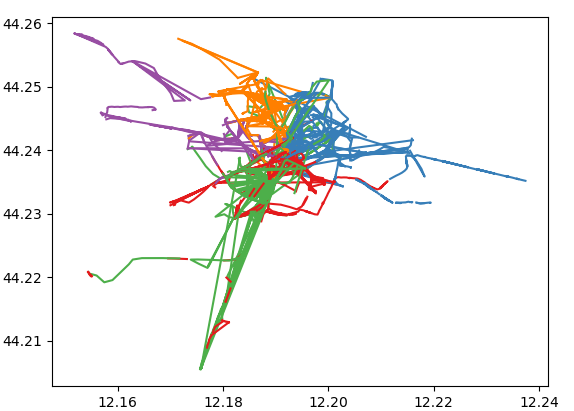
\includegraphics[width=\textwidth]{ward-agglomerative-plot}
		\caption{Silhouette: 0.28. Rentals showed: 200.}
		\label{fig:ward-agglomerative-line}
	\end{figure}
	\column{0.3\textwidth}
	\begin{figure}[bt]
		\centering
		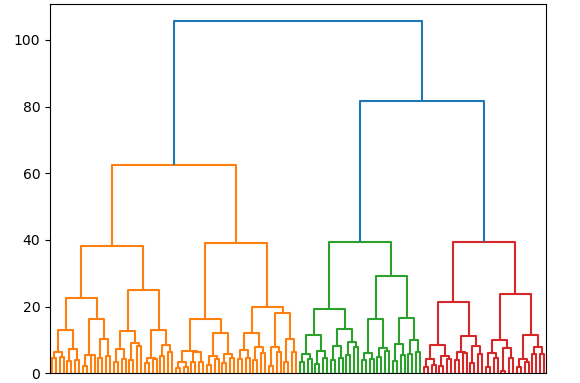
\includegraphics[width=\textwidth]{ward-agglomerative-dendrogram}
		\caption{Dendrogram up to level 5 of merge}
		\label{fig:ward-agglomerative-dendrogram}
	\end{figure}
\end{columns}
\end{frame}

\begin{frame}{K-Means clustering}
\begin{figure}[bt]
	\centering
	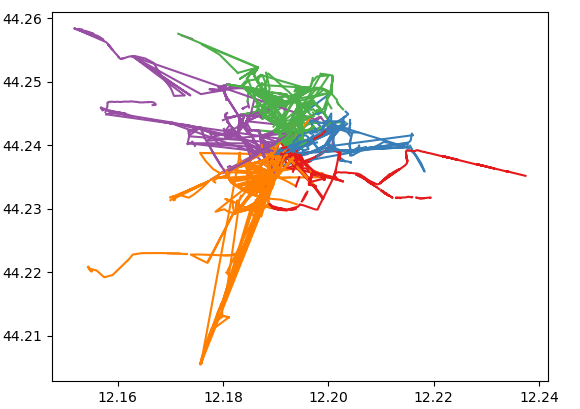
\includegraphics[width=0.85\textwidth]{k-means-plot}
	\caption{Silhouette: 0.352. Rentals showed: 200.}
	\label{fig:k-means-line}
\end{figure}
\end{frame}

\section{Conclusion}
\begin{frame}{Final considerations}
\begin{itemize}
	\item \textit{K-Means} best result in terms of plot representation and \textit{Silhouette score};
	\item Custom \textit{PCA} implementation results similar to traditional \textit{PCA} approach based on the $80\%$ of cumulative variance;
	\item Time useful for partition and group, but not for bottom-up clustering techniques;
	\item Clustering with \textit{PCA} shows better results in variance terms;
	\item Clustering with heuristic features maintains the rental information;
	\item Clustering has always to be performed on a specific region of interest in order to optimize the results;
	\item \textit{Silhouette score} is not a validation methodology so reliable, because it depends a lot on the data you are dealing with;
\end{itemize}
\end{frame}

\begin{frame}{K-Means slices}
\textit{K-Means} without \textit{PCA} with only latitude and longitude features.
\begin{figure}[bt]
	\centering
	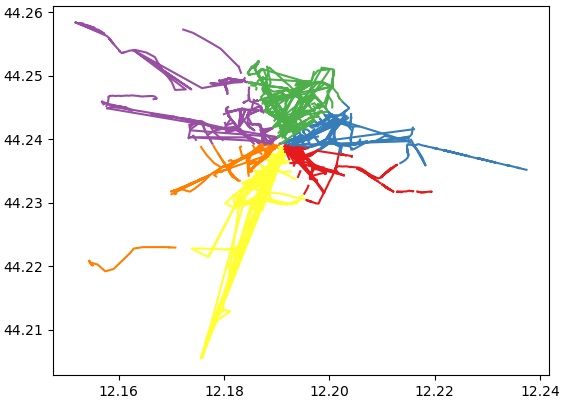
\includegraphics[width=0.80\columnwidth]{kmeans-without-pca}
	\label{fig:kmeans-without-pca}
\end{figure}
\end{frame}

\begin{frame}{K-Means bad result}
\textit{K-Means} with 5 clusters performed on all positions showed on one city.
\begin{figure}[bt]
	\centering
	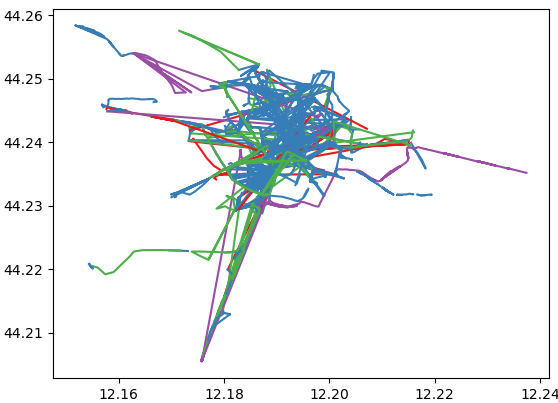
\includegraphics[width=0.80\columnwidth]{kmeans-bad}
	\label{fig:kmeans-bad}
\end{figure}
\end{frame}

\begin{frame}{K-Means 3D}
\begin{figure}[bt]
	\centering
	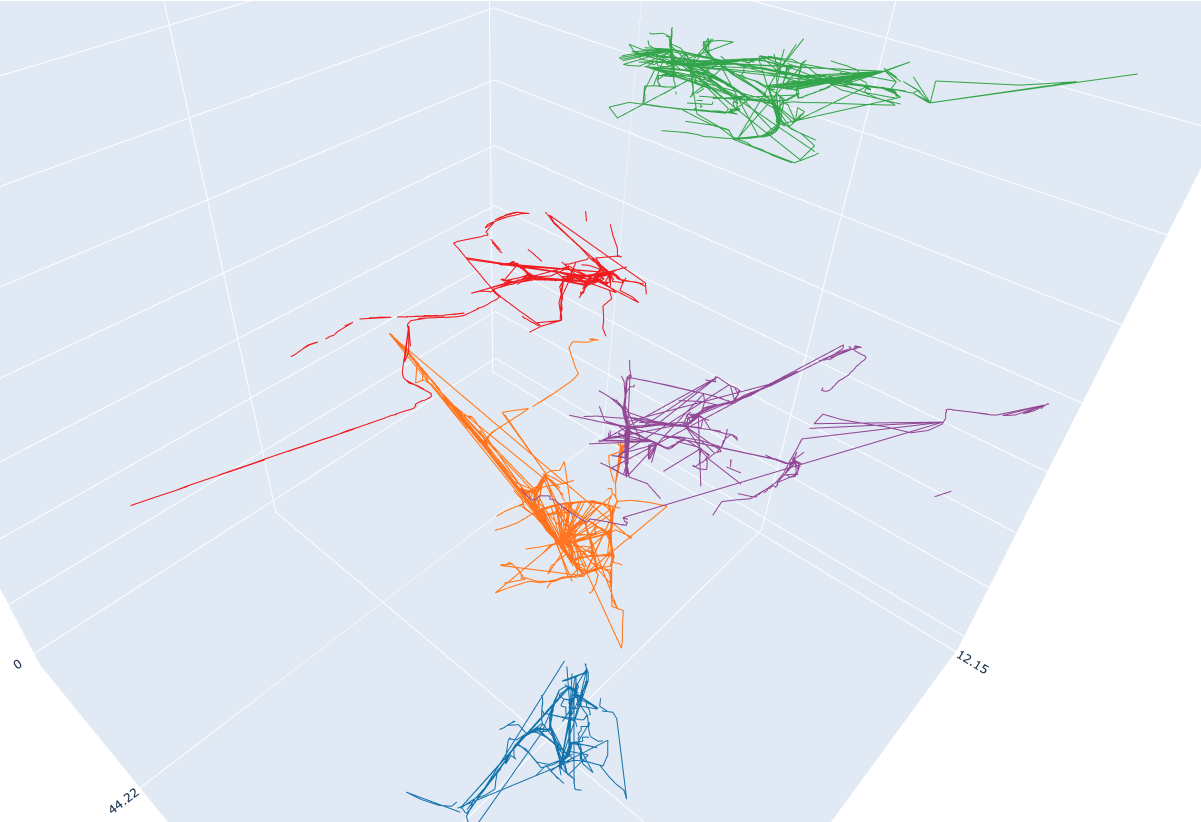
\includegraphics[width=\columnwidth]{kmeans-3d}
	\label{fig:kmeans-3d}
\end{figure}
\end{frame}

\end{document}